% \documentclass[12pt, twoside]{article}
\usepackage[letterpaper, margin=1in, headsep=0.2in]{geometry}
\setlength{\headheight}{0.6in}
%\usepackage[english]{babel}
\usepackage[utf8]{inputenc}
\usepackage{microtype}
\usepackage{amsmath}
\usepackage{amssymb}
%\usepackage{amsfonts}
\usepackage[nomessages]{fp} %\FPeval{\var-name}{2*sin(pi/6)}
\usepackage{siunitx} %units in math. eg 20\milli\meter
\usepackage{yhmath} % for arcs, overparenth command
\usepackage{tikz} %graphics
\usetikzlibrary{quotes, angles, arrows, arrows.meta}
\usepackage{graphicx} %consider setting \graphicspath{{images/}}
\usepackage{parskip} %no paragraph indent
\usepackage{enumitem}
\usepackage{multicol}
\usepackage{venndiagram}

\usepackage{fancyhdr}
\pagestyle{fancy}
\fancyhf{}
\renewcommand{\headrulewidth}{0pt} % disable the underline of the header
\raggedbottom
\hfuzz=2mm %suppresses overfull box warnings

\usepackage{hyperref}

\fancyhead[LE]{\thepage}
\fancyhead[RO]{\thepage \\ Name: \hspace{4cm} \,\\}
\fancyhead[LO]{BECA / Dr. Huson / Geometry\\*  Unit 6: Analytic geometry\\* 1 December 2022}

\begin{document}

\subsubsection*{6.7 Homework: Mixed review}
\begin{enumerate}
\item In the diagram below $\angle AOB = x-35$ and $\displaystyle \angle COD = \frac{3}{4}(x+55)$. Find $\angle BOC$. \vspace{0.25cm}
\begin{flushright}
\begin{tikzpicture}[scale=1, rotate=0]
\draw [<->, thick] (0,0)--(155:5);
\draw [<->, thick] (-5,0)--(5,0);
\draw [->, thick] (0,0)--(0,4);
\draw (0,0)++(0.3,0)--++(0,0.3)--+(-0.3,0);
%\draw [fill] (-1,2.5) circle [radius=0.05] node[left ]{$B$};
\draw [fill] (155:3) circle [radius=0.05] node[below left]{$B$};
\draw [fill] (-4,0) circle [radius=0.05] node[below]{$A$}; 
\draw [fill] (0,0) circle [radius=0.05] node[below]{$O$};
\draw [fill] (0,3) circle [radius=0.05] node[left]{$C$};
\draw [fill] (4,0) circle [radius=0.05] node[below]{$D$};
\end{tikzpicture}
\end{flushright}

\item In the diagram below $\angle AOB = 5x-15$ and $\angle DOE = 4x-4$. Find $m\angle AOB$. \vspace{0.25cm}
\begin{flushright}
\begin{tikzpicture}[scale=1.3, rotate=40]
  \draw [<->, thick] (-40:3)--(0,0)--(140:3);
  \draw [<->, thick] (-3,0)--(3,0);
  \draw [->, thick] (0,0)--(0,3);
  \draw (0,0)++(0.3,0)--++(0,0.3)--+(-0.3,0);
  %\draw [fill] (-1,2.5) circle [radius=0.05] node[left ]{$B$};
  \draw [fill] (140:2) circle [radius=0.05] node[below left]{$B$};
  \draw [fill] (-2,0) circle [radius=0.05] node[below]{$A$}; 
  \draw [fill] (0,0) circle [radius=0.05] node[below right]{$O$};
  \draw [fill] (0,2) circle [radius=0.05] node[below left]{$C$};
  \draw [fill] (2,0) circle [radius=0.05] node[below]{$D$};
  \draw [fill] (-40:2) circle [radius=0.05] node[below]{$E$};
\end{tikzpicture}
\end{flushright}

\newpage
\item In the following two problems, solve for the value of $x$.
  \begin{multicols}{2}
    \begin{enumerate}
      \item   $\frac{4}{3}(6x-3)=x + 10$
      \item   $\frac{2}{5}(x-1)+\frac{5}{2}(1-x)=0$
    \end{enumerate}
  \end{multicols}
  \vspace{6cm}

\item Given the linear function $f(x)=-2x+14$.
\begin{multicols}{2}
  \begin{enumerate}
    \item Find $f(4)$
    \item   $f(x)=21$. Find $x$.
  \end{enumerate}
\end{multicols} \vspace{4cm}

\item Given two lines $\displaystyle f(x)=\frac{3}{2}x+8$ and $\displaystyle g(x)=-\frac{1}{4}x+5\frac{1}{2}$. Is the point $P(-2,5)$ on one line, both, or neither? \vspace{4cm} 

\item The line $l$ is graphed at right.
\begin{multicols}{2}
\begin{enumerate}
  \item Write down the line's slope.\\ $m=$
  \vspace{0.5cm}
  \item Write down it's $y$-intercept.\\ $b=$
  \vspace{0.5cm}
  \item Write down the equation of the line.
  \vspace{1.5cm}
  \item Draw a line parallel to $l$ through point $P$. (use a straight edge for full credit)
\end{enumerate} \vspace{.5cm}
  \begin{center} 
  \begin{tikzpicture}[scale=0.8]
    \draw [help lines] (-2,-1) grid (5,6);
    \draw [thick, ->] (-2.2,0) -- (5.4,0) node [below right] {$x$};
    \draw [thick, ->] (0,-1.2)--(0,6.4) node [left] {$y$};
    \foreach \x in {-2,-1,1,2,...,5} \draw (\x cm,1pt) -- (\x cm,-1pt) node[anchor=north] {$\x$};
    \foreach \y in {1, 2, 3, 4, 5} \draw (1pt,\y cm) -- (-1pt,\y cm) node[anchor=east] {$\y$};
    \draw [thick, <->] (-1.5,2.75) -- (4.5,-0.25)node[below]{$l$};
    \fill (2,4) circle[radius=0.1] node[above right]{$P$};
  \end{tikzpicture}
  \end{center}
\end{multicols}

\item Find the slope of the line through the points $(2, -2)$ and $(-1, 4)$. \vspace{4cm}

\item Write the linear equation $\displaystyle y-7=\frac{3}{2}(x+10)$ in the form $y=mx+c$. \vspace{4cm}

\item Is the point $(-5,1)$ on the line $\displaystyle y=-\frac{3}{5}x-3$? Support your answer algebraically.

\newpage
\item Two lines are graphed below. 
\begin{enumerate}
  \item Complete the T-tables for each.
  \item Write down the equations for each.
\end{enumerate}
  \begin{center} 
  \begin{tikzpicture}[scale=0.8]
    \draw [help lines] (-3,-2) grid (6,6);
    \draw [thick, ->] (-3.2,0) -- (6.4,0) node [below right] {$x$};
    \draw [thick, ->] (0,-2.2)--(0,6.4) node [right] {$y$};
    \foreach \x in {-3,-2,-1,1,2,...,6} \draw (\x cm,1pt) -- (\x cm,-1pt) node[anchor=north] {$\x$};
    \foreach \y in {-1,1, 2, 3, 4, 5,6} \draw (1pt,\y cm) -- (-1pt,\y cm) node[anchor=east] {$\y$};

    \draw [thick, <->,samples=20,domain=-2.5:4.5] plot(\x,0.5*\x+4);
    \node at (4.5,5.5){$f$};
    \draw [thick, <->,samples=20,domain=-0.4:2.5] plot(\x,3*\x-1);
    \node at (2,6.5){$g$};

    \draw [thick] (-7,-1) -- (-7,6);
    \draw [thick] (-8.5,5) -- (-5.5,5);
    \node at (-7,7){$f(x)$};
    \node at (-8,5.5){$x$};
    \node at (-6,5.5){$y$};
    \draw [thick] (9,-1) -- (9,6);
    \draw [thick] (7.5,5) -- (10.5,5);
    \node at (9,7){$g(x)$};
    \node at (-8,4){$-2$}; 
    \node at (-8,2.5){$0$}; 
    \node at (-6,1){$5$}; 
    \node at (-6,-0.5){$6$};
    \fill (-2,3) circle[radius=0.1];
    \fill (0,4) circle[radius=0.1];
    \fill (2,5) circle[radius=0.1];
    \fill (4,6) circle[radius=0.1];
  \end{tikzpicture}
  \end{center} \vspace{1cm}


\end{enumerate}
\end{document}